\documentclass[10pt, a5paper]{article}
\usepackage{pdfpages}
\usepackage{parallel}
\usepackage[T2A]{fontenc}
\usepackage{ucs}
\usepackage[utf8x]{inputenc}
\usepackage[polish,english,russian]{babel}
\usepackage{hyperref}
\usepackage{rotating}
\usepackage[inner=2cm,top=1.8cm,outer=2cm,bottom=2.3cm,nohead]{geometry}
\usepackage{listings}
\usepackage{graphicx}
\usepackage{wrapfig}
\usepackage{longtable}
\usepackage{indentfirst}
\usepackage{array}
\newcolumntype{P}[1]{>{\raggedright\arraybackslash}p{#1}}
\frenchspacing
\usepackage{fixltx2e} %text sub- and superscripts
\usepackage{icomma} % коскі ў матэматычным рэжыме
\PreloadUnicodePage{4}

\newcommand{\longpage}{\enlargethispage{\baselineskip}}
\newcommand{\shortpage}{\enlargethispage{-\baselineskip}}

\def\switchlang#1{\expandafter\csname switchlang#1\endcsname}
\def\switchlangbe{
\let\saverefname=\refname%
\def\refname{Літаратура}%
\def\figurename{Іл.}%
}
\def\switchlangen{
\let\saverefname=\refname%
\def\refname{References}%
\def\figurename{Fig.}%
}
\def\switchlangru{
\let\saverefname=\refname%
\let\savefigurename=\figurename%
\def\refname{Литература}%
\def\figurename{Рис.}%
}

\hyphenation{admi-ni-stra-tive}
\hyphenation{ex-pe-ri-ence}
\hyphenation{fle-xi-bi-li-ty}
\hyphenation{Py-thon}
\hyphenation{ma-the-ma-ti-cal}
\hyphenation{re-ported}
\hyphenation{imp-le-menta-tions}
\hyphenation{pro-vides}
\hyphenation{en-gi-neering}
\hyphenation{com-pa-ti-bi-li-ty}
\hyphenation{im-pos-sible}
\hyphenation{desk-top}
\hyphenation{elec-tro-nic}
\hyphenation{com-pa-ny}
\hyphenation{de-ve-lop-ment}
\hyphenation{de-ve-loping}
\hyphenation{de-ve-lop}
\hyphenation{da-ta-ba-se}
\hyphenation{plat-forms}
\hyphenation{or-ga-ni-za-tion}
\hyphenation{pro-gramming}
\hyphenation{in-stru-ments}
\hyphenation{Li-nux}
\hyphenation{sour-ce}
\hyphenation{en-vi-ron-ment}
\hyphenation{Te-le-pathy}
\hyphenation{Li-nux-ov-ka}
\hyphenation{Open-BSD}
\hyphenation{Free-BSD}
\hyphenation{men-ti-on-ed}
\hyphenation{app-li-ca-tion}

\def\progref!#1!{\texttt{#1}}
\renewcommand{\arraystretch}{2} %Іначай формулы ў матрыцы зліпаюцца з лініямі
\usepackage{array}

\def\interview #1 (#2), #3, #4, #5\par{

\section[#1, #3, #4]{#1 -- #3, #4}
\def\qname{LVEE}
\def\aname{#1}
\def\q ##1\par{{\noindent \bf \qname: ##1 }\par}
\def\a{{\noindent \bf \aname: } \def\qname{L}\def\aname{#2}}
}

\def\interview* #1 (#2), #3, #4, #5\par{

\section*{#1\\{\small\rm #3, #4. #5}}

\def\qname{LVEE}
\def\aname{#1}
\def\q ##1\par{{\noindent \bf \qname: ##1 }\par}
\def\a{{\noindent \bf \aname: } \def\qname{L}\def\aname{#2}}
}

\begin{document}
\title{Zotero: аўтаматычная бібліяграфія ў WYSIWYG"=рэдактарах}
\author{Антон Літвіненка, Кіеў, Украiна\footnote{\url{tenebrosus.scriptor@gmail.com}, \url{http://lvee.org/en/abstracts/127}}}
\maketitle
\begin{abstract}
Automatic bibliography generation, being common for LaTeX users, is irrationally rarely used by scientists that prepare publica\-tions via WYSIWYG editing packages. While some linkers of BibTeX system to office packages exist, one may prefer more profound reference systems that automatize also crawling and managing citations as well as regular sorting and pattern format\-ting. FLOSS example of such system, named Zotero, is discussed in the presentation.
\end{abstract}
\subsection*{Матывацыя ды патрабаванні}

Афармленне вынікаў навуковых даследванняў у выглядзе артыкулаў, манаграфій ды іншых працаў, патрабуе афармлення спісу літаратуры пад пэўныя патрабаванні. Гэтыя патрабаванні, як правіла, ўключаюць нумерацыю спасылак на літаратурныя крыніцы ў парадку іхняга ўзнікнення ў тэксце працы, а таксама фарматаванне тэксту спасылкі паводле пэўнага шаблону, які адрозніваецца ў розных рэдакцыях. Парадак узнікнення можа істотна мяняцца пад час працы над тэкстам, рознасць шаблонаў афармлення замінае ўжытку спасылак з аднаго артыкулу пры напісанні іншага. Ручная перанумероўка ды перафарматаванне спасылак з’яўляецца маруднай працай, якая лёгка прыводзіць да памылак.

У выдавецкіх сістэмах на базе LaTeX сродкі аўтаматычнага фарматавання з’яўляюцца тыповай і неад’ёмнай часткай сістэмы. Уключэнне спасылкі рэалізуецца праз адпаведную каманду працэсара. У выпадку WYSIWYG"=працэсараў падобны функцыянал даводзіцца рэалізоўваць праз вонкавую сістэму ды плагіны для ёйнай інтэграцыі з тэкставым працэсарам. З улікам адсутнасці тэкставых камандаў патрэбныя адмысловыя аб’екты для захавання дадзеных спасылкі (у выпадку OpenOffice ужываюцца зноскі (reference marks) альбо закладкі (bookmarks), ў MS Word "--- палі (fields) альбо закладкі (bookmarks).

\subsection*{Кампаненты Zotero}

\begin{enumerate}
  \item Сістэма імпарту спасылак. Дазваляе дадаць спасылку да бібліяграфічнай базы ``адным націскам'' са старонкі навуковага часопісу ці сістэмы пошуку навуковай літаратуры, альбо праз зазначэнне DOI, ISBN, Pubmed ID і г.д., а таксама з іншых бібліяграфічных базаў (напрыклад, базы для BibTeX).
  \item Арганізатар бібліяграфічнай базы. Дазваляе ствараць, выдаляць, рэдагаваць і сартаваць спасылкі, а таксама арганізуе сінхранізацыю праз анлайн"=сховішча.
  \item Плагін інтэграцыі з тэкставым працэсарам.
  \item Дадатковыя кампаненты.
\end{enumerate}

\subsection*{CSL. Рэпазіторыі стыляў}

Фарматаванне тэксту спасылкі задаецца шаблонам, апісаным з дапамогай адмысловае мовы CSL (Citation Style Language), што базуецца на мове разметкі XML \cite{Litvinenko1}. Напрыклад, фрагмент апісання стылю Journal of American Chemical Society выглядае наступным чынам:

\begin{verbatim}
<if type="article-magazine">
         <group delimiter=" ">
           <text variable="container-title" font-style=
"italic" suffix="."/>
           <text macro="edition"/>
           <text macro="publisher"/>
           <text macro="full-issued" suffix=","/>
           <text macro="pages"/>
         </group>
       </if>
       <else-if type="thesis">
         <group delimiter=", ">
           <group delimiter=". ">
             <text variable="title"/>
             <text variable="genre"/>
           </group>
           <text macro="publisher"/>
           <text macro="issued"/>
           <text macro="volume"/>
           <text macro="pages"/>
         </group>
       </else-if>
\end{verbatim}

За час існавання праэкту напрацавана вялікая колькасць стыляў для разнастайных навуковых часопісаў, якія можна знайсці ў адмысловым рэпазіторыі \cite{Litvinenko2}. У выпадку, калі патрэбнага стылю бракуе, яго можна стварыць уласнаруч праз адаптацыю наяўных. Для гэтага распрацаваны візуальны рэдактар (рыс. 1), які дазваляе паводле прыкладу спасылкі знайсці найбольш падобны стыль і змяніць яго пад свае патрэбы, не кранаючы XML"=код  \cite{Litvinenko3}.

\begin{figure}[h!]
  \centering
  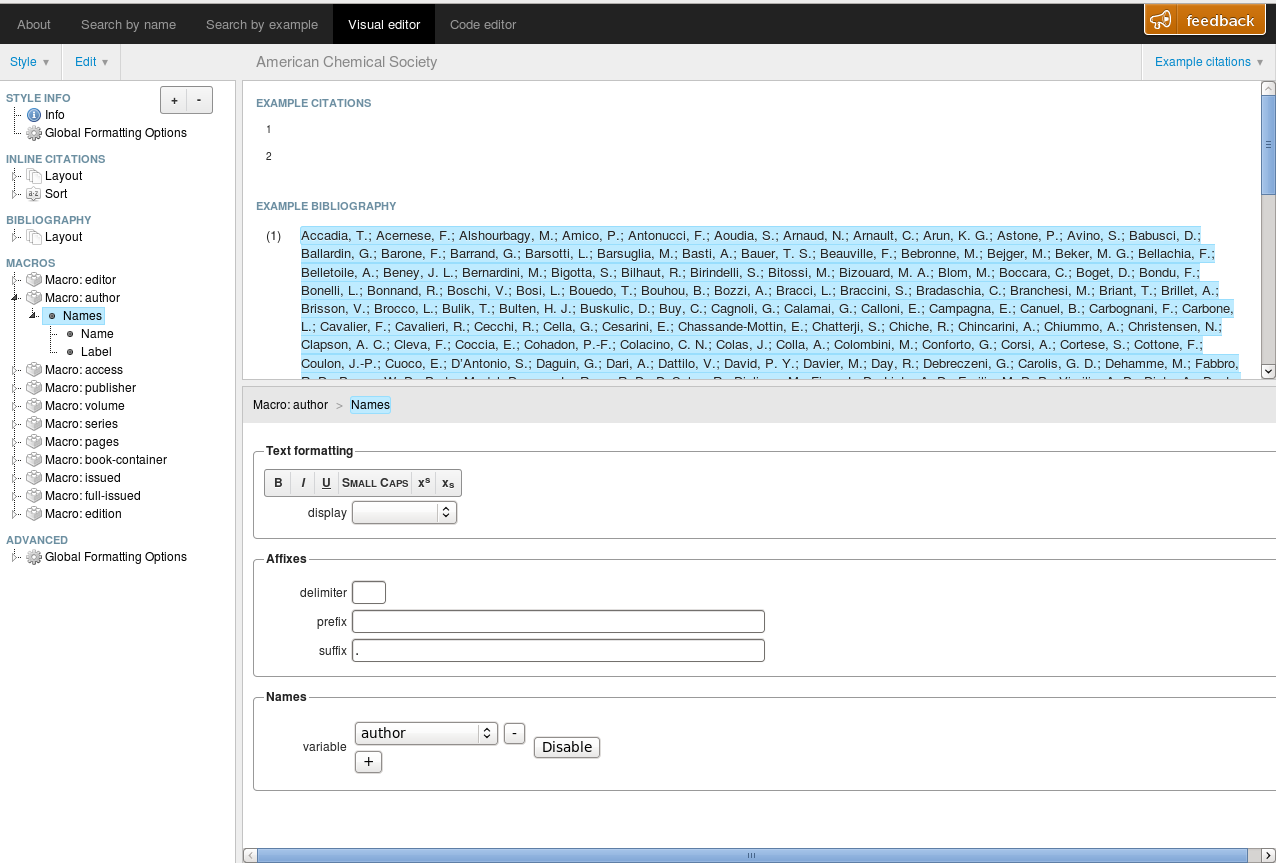
\includegraphics[scale=0.2]{11_2014_screen_editor.png}
  \caption{Акно візуальнага рэдактара: фарматаванне імёнаў аўтараў}
\end{figure}

\subsection*{Практычнае выкарыстанне}

Zotero рэалізаваны ў выглядзе плагіна для Firefox (найбольш поўнафункцыянальны) ды standalone"=праграмы.

\subsubsection*{Напаўненне базы бібліяграфіі}

Найбольш тыповы і зручны спосаб для артыкулаў: зайсці на старонку з анатацыяй адпаведнага артыкулу на афіцыйным сайце часопісу і націснуць кнопку захавання спасылкі (рыс. 2).

Для кніг: ўвесці ISBN.

\subsubsection*{Кіраванне базай}

Спасылкі сартуюцца па тэках (адна спасылка можа знаходзіцца ў некалькіх тэках). Акно плагіна адлюстроўвае спіс тэкаў, спіс спасылак у абранай тэцы ды падрабязнасці абранай спасылкі (рыс. 1). Магчымы хуткі пошук па зместу спасылак.


\begin{figure}[h!]
  \centering
  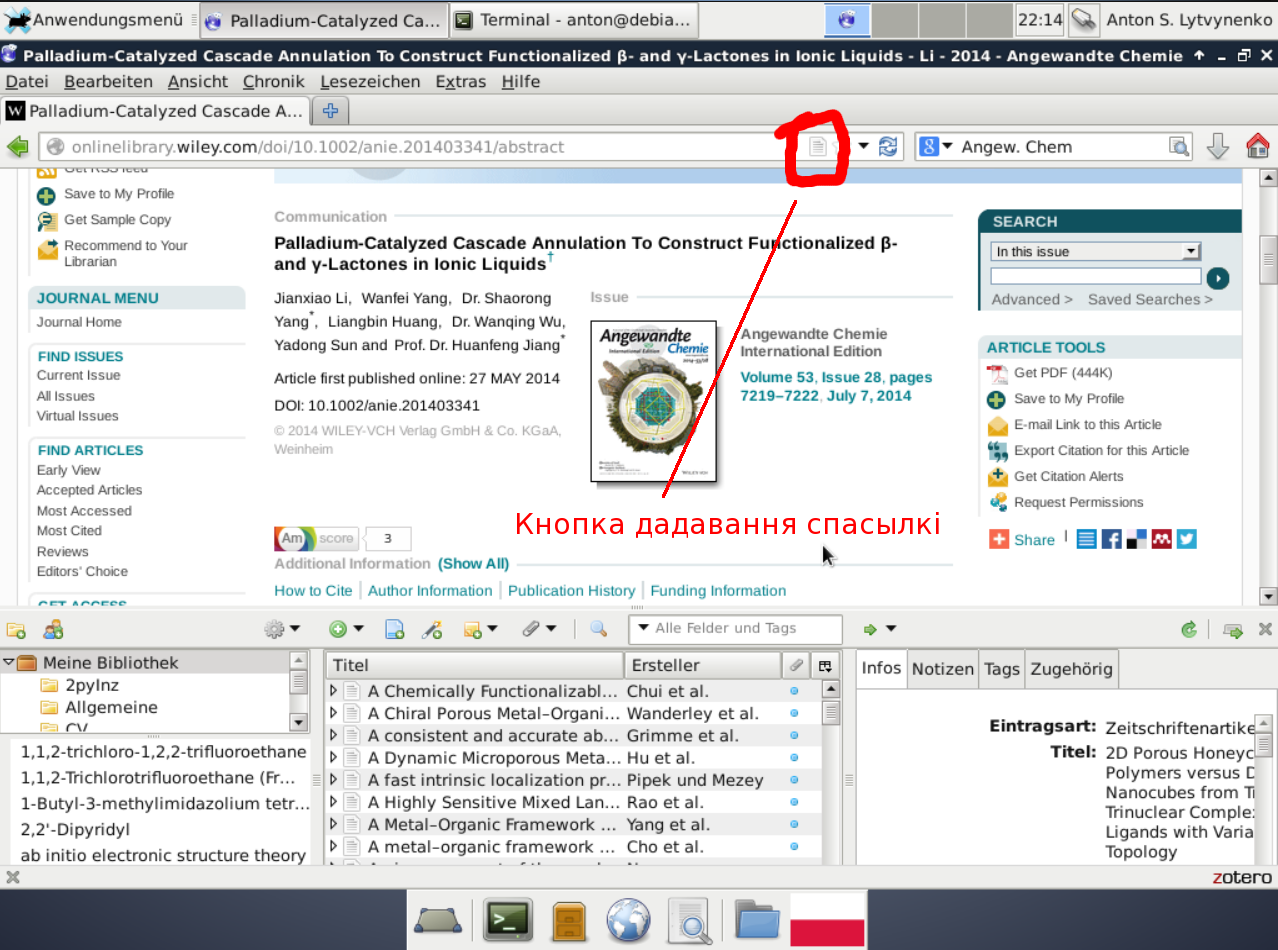
\includegraphics[scale=0.2]{11_2014_Fig1.png}
  \caption{Панэль Firefox"=плагіна Zotero і аўтаматычнае дадаванне спасылкі са старонкі часопіса Angewandte Chemie}
\end{figure}



\subsubsection*{Дадаванне спасылкі ў тэкст}

Інтэграцыйны плагін дадае кнопкі ў панэль офіснага працэсара (рыс. 3): дадаць спасылку (пад час першага выкарыстання прапануецца выбраць шаблон фарматавання), рэдагаваць спасылку, дадаць спіс літаратуры, рэдагаваць спіс літаратуры, панавіць спіс, усталяваць опцыі для дакуманту, выдаліць коды палёў (пераўтварае фарматаваныя спасылкі ў звыклы тэкст). Устаўка ды рэдагаванне магчымае праз выбар спасылак са спісаў, а таксама праз хуткі пошук у акенцы дадавання (рыс. 4) Выдаленне спасылкі "--- праз выдаленне адпаведнага аб’екту ў тэксце.



\begin{figure}[h!]
  \centering
  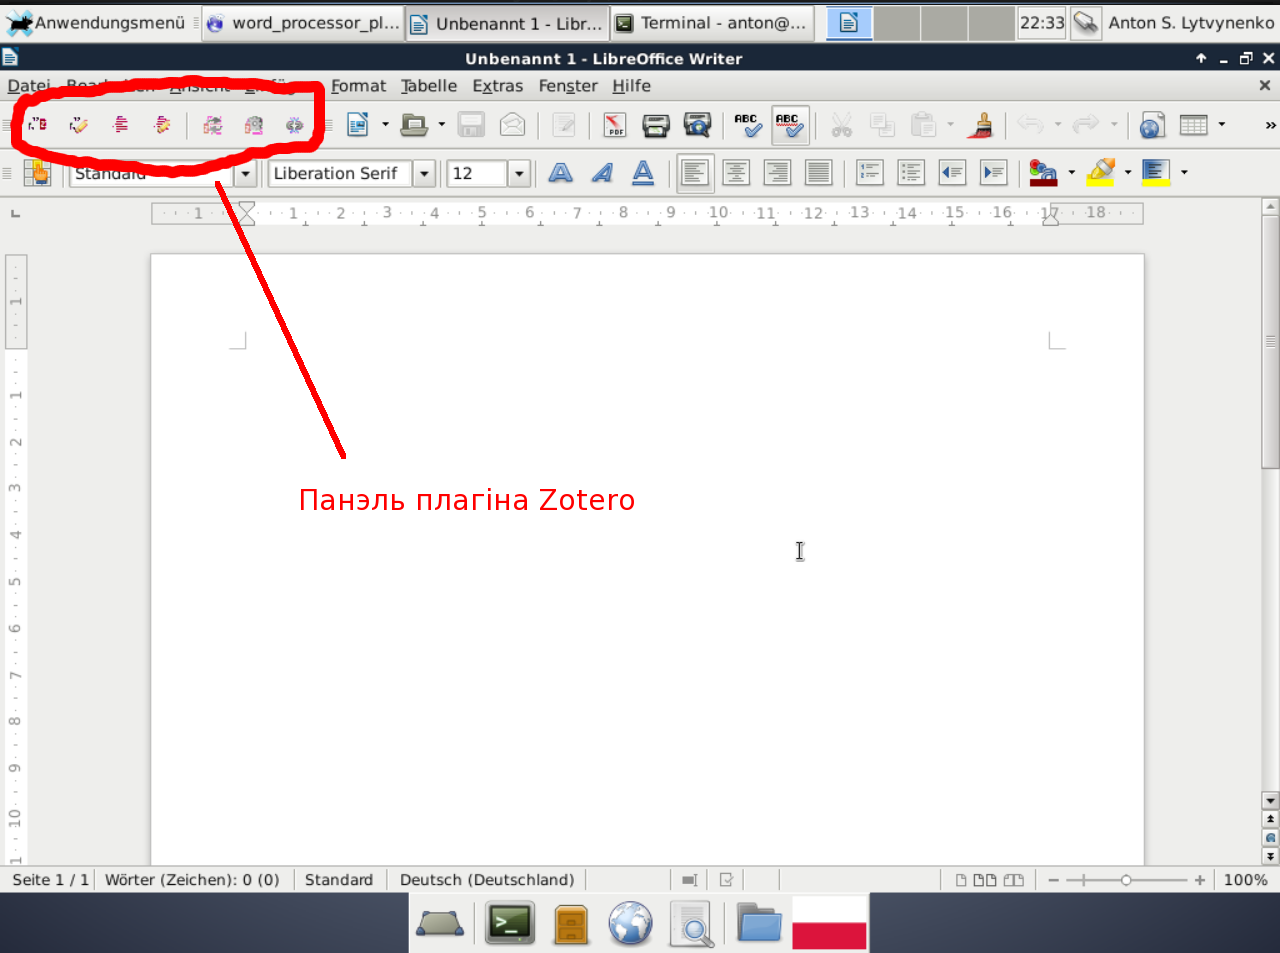
\includegraphics[scale=0.2]{11_2014_Fig2.png}
  \caption{Інтэграцыя Zotero ў LibreOffice}
\end{figure}


\begin{figure}[h!]
  \centering
  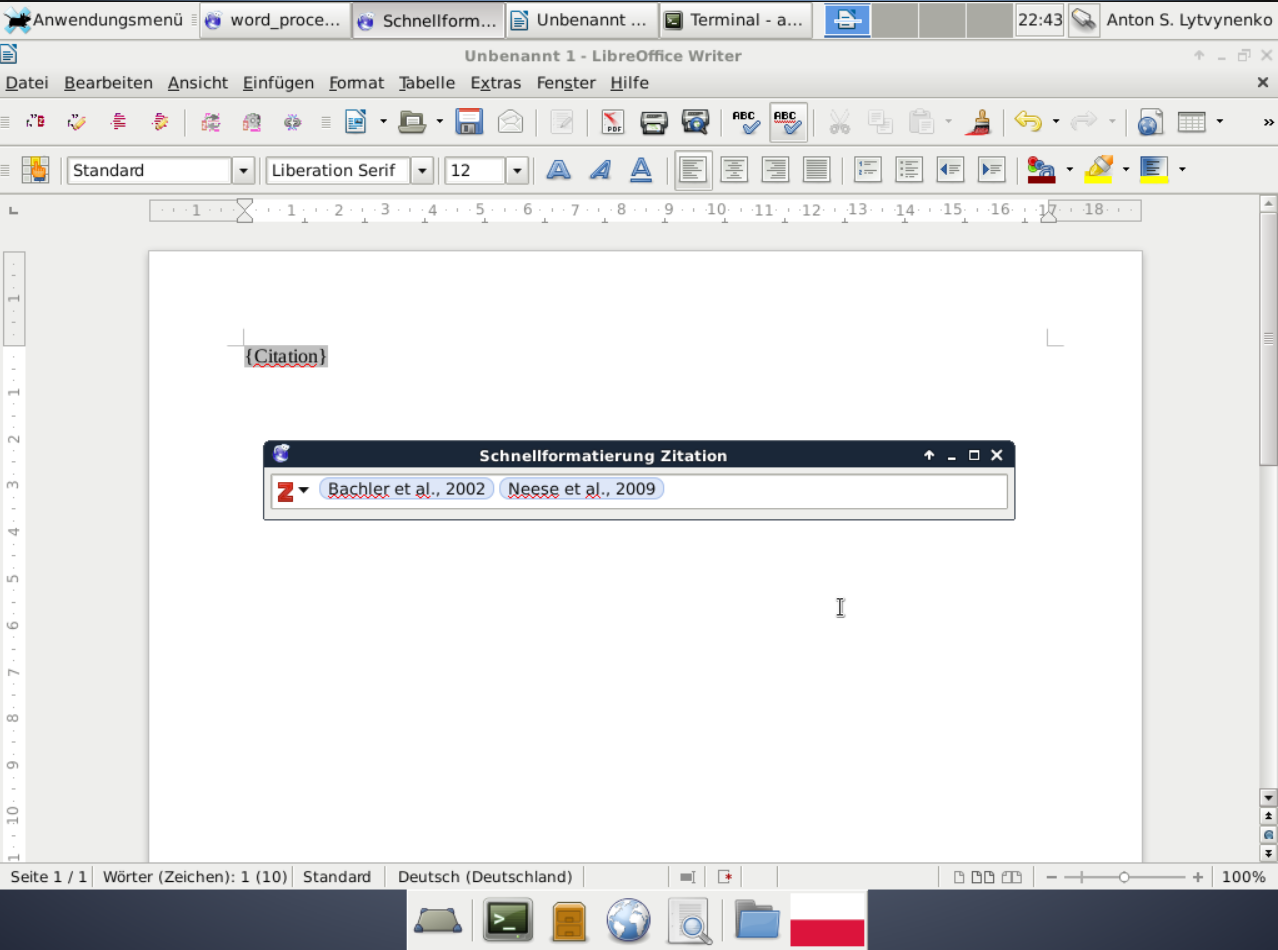
\includegraphics[scale=0.2]{11_2014_Fig3.png}
  \caption{Устаўка спасылкі хуткім пошукам}
\end{figure}

\subsection*{Палі і закладкі. Copy/Paste/Delete. Абмен \linebreak Open/Libre Office ды MS}

Zotero можа захоўваць дадзеныя пра спасылку ў зносках/палях альбо закладках. Варыянт закладак забяспечвае сумяшчальнасць пры супольнай працы ў OpenOffice ды MS Word, але не дазваляе аперацыі капіявання"=ўстаўкі над спасылкамі ў тэксце. Больш стандартным рэжымам з’яўляецца выкарыстанне зносак/палёў, якія дазваляюць працу са спасылкамі як са звыклымі элементамі тэксту "--- капіяванне, ўстаўка, перанос (у тым ліку з файлу ў файл).

\subsection*{Некаторыя брудныя падрабязнасці}

Іншы раз Zotero праз тыя ці іншыя прычыны фарматуе спасылку няправільна. Асабліва часта гэта стаецца пры наяўнасці ў спасылцы верхніх і ніжніх індэксаў, якія адлюстроўваюцца без адпаведнага фарматавання. Магчымасць ``рэдагаваць бібліяграфію'' дазваляе адфарматаваць тэкст спасылкі ў спісе літаратуры ўручную. Пры гэтым яе тэкст (а таксама нумар, зазначаны ў спісе літаратуры) прыпыняе абнаўляцца аўтаматычна (нумар у асноўным тэксце абнаўляецца) "--- пажадана не забыцца на гэта ў фінальнай версіі дакуманта.

Магчымасць ручнога фарматавання дае таксама магчымасць розных нестандартных спасылак (напрыклад, кампазітнай спасылкі, пры якой пад адным нумарам цытуецца некалькі спасылак (a, b, \ldots{})). Карыстальнік можа спачатку згенераваць праз сістэму індывідуальныя спасылкі, пасля стварыць спасылку на нейкі dummy"=аб’ект (напрыклад, нататку), спаслацца на яго і адфарматаваць тэкст уручную, ўставіўшы згенераваны тэкст пасля адпаведнага рэдагавання.

Над дакументам, у які з дапамогай Zotero ўстаўленыя спасылкі, можна працаваць і на кампутарах, дзе Zotero не ўсталявана, ў тым ліку ў версіях рэдактараў, якія не падтрымліваюцца Zotero (напрыклад, MS Word раней за версію 2003), ў тым ліку выконваць аперацыі капіявання, пераносу ці выдалення спасылак у тэксце. Пасля рэдагавання на такой сістэме дастаткова адчыніць дакумант у сістэме з усталяваным Zotero і панавіць бібліяграфію.

\subsection*{Высновы}

FLOSS"=сістэма Zotero, што інтэгруецца ў папулярныя офісныя тэкставыя працэсары, дазваляе аўтаматычнае фарматаванне і перанумероўку спасылак на літаратурныя крыніцы, што істотна палягшае працу навукоўцаў пры афармленні вынікаў іхняе працы. У адрозненні ад працы BibTeX і заснаваных на ім сістэм, Zotero дапоўненая кампанентамі аўтаматызаванага збору ды арганізацыі бібліяграфічных спасылак, што з’яўляецца мэтазгодным для \linebreak WYSIWYG"=сістэмы і таксама палягшае працу.

\begin{thebibliography}{9}
\bibitem{Litvinenko1} \url{http://citationstyles.org/}
\bibitem{Litvinenko2} \url{https://www.zotero.org/styles}
\bibitem{Litvinenko3} \url{http://editor.citationstyles.org/searchByExample/}
\end{thebibliography}
\end{document}
